\documentclass[11pt,a4paper]{article}
%%%%%%%%%%%%%%%%%%%%%%%%% Credit %%%%%%%%%%%%%%%%%%%%%%%%

% template ini dibuat oleh martin.manullang@if.itera.ac.id untuk dipergunakan oleh seluruh sivitas akademik itera.

%%%%%%%%%%%%%%%%%%%%%%%%% PACKAGE starts HERE %%%%%%%%%%%%%%%%%%%%%%%%
\usepackage{graphicx}
\usepackage{caption}
\usepackage{microtype}
\captionsetup[table]{name=Tabel}
\captionsetup[figure]{name=Gambar}
\usepackage{tabulary}
\usepackage{minted}
\usepackage{lmodern}
\usepackage{amsmath}
\usepackage{fancyhdr}
\usepackage{amssymb}
\usepackage{amsthm}
\usepackage{placeins}
\usepackage{amsfonts}
\usepackage{graphicx}
\usepackage[all]{xy}
\usepackage{tikz}
\usepackage{verbatim}
\usepackage[left=2cm,right=2cm,top=3cm,bottom=2.5cm]{geometry}
\usepackage{hyperref}
\hypersetup{
    colorlinks,
    linkcolor={red!50!black},
    citecolor={blue!50!black},
    urlcolor={blue!80!black}
}
\usepackage{caption}
\usepackage{subcaption}
\usepackage{multirow}
\usepackage{psfrag}
\usepackage[T1]{fontenc}
\usepackage[scaled]{beramono}
% Enable inserting code into the document
\usepackage{listings}
\usepackage{xcolor} 
% custom color & style for listing
\definecolor{codegreen}{rgb}{0,0.6,0}
\definecolor{codegray}{rgb}{0.5,0.5,0.5}
\definecolor{codepurple}{rgb}{0.58,0,0.82}
\definecolor{backcolour}{rgb}{0.95,0.95,0.92}
\definecolor{LightGray}{gray}{0.9}
\lstdefinestyle{mystyle}{
	backgroundcolor=\color{backcolour},   
	commentstyle=\color{green},
	keywordstyle=\color{codegreen},
	numberstyle=\tiny\color{codegray},
	stringstyle=\color{codepurple},
	basicstyle=\ttfamily\footnotesize,
	breakatwhitespace=false,         
	breaklines=true,                 
	captionpos=b,                    
	keepspaces=true,                 
	numbers=left,                    
	numbersep=5pt,                  
	showspaces=false,                
	showstringspaces=false,
	showtabs=false,                  
	tabsize=2
}
\lstset{style=mystyle}
\renewcommand{\lstlistingname}{Kode}
%%%%%%%%%%%%%%%%%%%%%%%%% PACKAGE ends HERE %%%%%%%%%%%%%%%%%%%%%%%%


%%%%%%%%%%%%%%%%%%%%%%%%% Data Diri %%%%%%%%%%%%%%%%%%%%%%%%
\newcommand{\student}{\textbf{Elma Nurul Fatika (122140069)}}     
\newcommand{\course}{\textbf{Sistem Teknologi Multimedia (IF25-40305)}}
\newcommand{\assignment}{\textbf{Worksheet 1: Setup Python Environment untuk Multimedia}}

%%%%%%%%%%%%%%%%%%% using theorem style %%%%%%%%%%%%%%%%%%%%
\newtheorem{thm}{Theorem}
\newtheorem{lem}[thm]{Lemma}
\newtheorem{defn}[thm]{Definition}
\newtheorem{exa}[thm]{Example}
\newtheorem{rem}[thm]{Remark}
\newtheorem{coro}[thm]{Corollary}
\newtheorem{quest}{Question}[section]
%%%%%%%%%%%%%%%%%%%%%%%%%%%%%%%%%%%%%%%%
\usepackage{lipsum}%% a garbage package you don't need except to create examples.
\usepackage{fancyhdr}
\pagestyle{fancy}
\lhead{Elma Nurul Fatika (122140069)}
\rhead{ \thepage}
\cfoot{\textbf{Worksheet 1: Setup Python Environment untuk Multimedia}}
\renewcommand{\headrulewidth}{0.4pt}
\renewcommand{\footrulewidth}{0.4pt}

%%%%%%%%%%%%%%  Shortcut for usual set of numbers  %%%%%%%%%%%

\newcommand{\N}{\mathbb{N}}
\newcommand{\Z}{\mathbb{Z}}
\newcommand{\Q}{\mathbb{Q}}
\newcommand{\R}{\mathbb{R}}
\newcommand{\C}{\mathbb{C}}
\setlength\headheight{14pt}

%%%%%%%%%%%%%%%%%%%%%%%%%%%%%%%%%%%%%%%%%%%%%%%%%%%%%%%555
\begin{document}
\thispagestyle{empty}
\begin{center}
	
\includegraphics[scale = 0.15]{Figure/ifitera-header.png}
	\vspace{0.1cm}
\end{center}
\noindent
\rule{17cm}{0.2cm}\\[0.3cm]
Nama: \student \hfill Tugas Ke: \assignment\\[0.1cm]
Mata Kuliah: \course \hfill Tanggal: \today\\
\rule{17cm}{0.05cm}
\vspace{0.1cm}



%%%%%%%%%%%%%%%%%%%%%%%%%%%%%%%%%%%%%%%%%%%%% BODY DOCUMENT %%%%%%%%%%%%%%%%%%%%%%%%%%%%%%%%%%%%%%%%%%%%%
\section{Tujuan Pembelajaran}
Setelah menyelesaikan worksheet ini, mahasiswa diharapkan mampu:
\begin{itemize}
    \item Memahami pentingnya manajemen environment Python untuk pengembangan multimedia
    \item Menginstall dan mengkonfigurasi Python environment menggunakan conda, venv, atau uv
    \item Menginstall library-library Python yang diperlukan untuk multimedia processing
    \item Memverifikasi instalasi dengan mengimpor dan menguji library multimedia
    \item Mendokumentasikan proses konfigurasi dan hasil pengujian dalam format \LaTeX
\end{itemize}

\section{Latar Belakang}
Python telah menjadi bahasa pemrograman yang sangat populer untuk multimedia processing karena memiliki ekosistem library yang sangat kaya. Namun, untuk dapat bekerja dengan multimedia secara efektif, kita perlu mengatur environment Python dengan benar dan menginstall library-library yang tepat.

Manajemen environment Python sangat penting untuk:
\begin{itemize}
    \item Menghindari konflik antar library (dependency conflict)
    \item Memastikan reproducibility dari project
    \item Memudahkan kolaborasi antar developer
    \item Memisahkan project yang berbeda dengan requirement yang berbeda
\end{itemize}

\section{Instruksi Tugas}

\subsection{Persiapan}
\textbf{Sebelum memulai, pastikan Anda telah:}
\begin{itemize}
    \item Menginstall Python 3.8 atau lebih baru di sistem Anda
    \item Memilih salah satu tool manajemen environment: \textbf{conda}, \textbf{venv}, atau \textbf{uv}
    \item Membuka terminal/command prompt
    \item Menyiapkan dokumen \LaTeX\ ini untuk dokumentasi
\end{itemize}

\subsection{Bagian 1: Membuat Environment Python}
Pilih \textbf{SALAH SATU} dari tiga opsi berikut dan ikuti langkah-langkahnya:

\subsubsection{Opsi 1: Menggunakan Conda (Direkomendasikan untuk pemula)}
Jalankan perintah berikut di terminal:

\begin{lstlisting}[language=bash, caption=Membuat environment dengan Conda]
# Membuat environment baru dengan nama 'multimedia'
conda create -n multimedia python=3.11

# Mengaktifkan environment
conda activate multimedia

# Verifikasi environment aktif
conda info --envs
\end{lstlisting}

\subsubsection{Opsi 2: Menggunakan venv (Built-in Python)}
\begin{lstlisting}[language=bash, caption=Membuat environment dengan venv]
# Membuat environment baru
python3 -m venv multimedia-env

# Mengaktifkan environment (Linux/Mac)
source multimedia-env/bin/activate

# Mengaktifkan environment (Windows)
# multimedia-env\Scripts\activate

# Verifikasi environment aktif
which python
\end{lstlisting}

\subsubsection{Opsi 3: Menggunakan uv (Modern dan cepat)}
\begin{lstlisting}[language=bash, caption=Membuat environment dengan uv]
# Install uv terlebih dahulu jika belum ada
# pip install uv

# Membuat environment baru
uv venv multimedia-uv

# Mengaktifkan environment (Linux/Mac)
source multimedia-uv/bin/activate

# Mengaktifkan environment (Windows)
# multimedia-uv\Scripts\activate

# Verifikasi environment aktif
which python
\end{lstlisting}

\textbf{Dokumentasikan di sini:}
\begin{itemize}
    \item Tool manajemen environment yang Anda pilih: \textbf{[Opsi 3, menggunakan uv]}
    \item Screenshot atau copy-paste output dari perintah verifikasi environment
    \begin{center}
	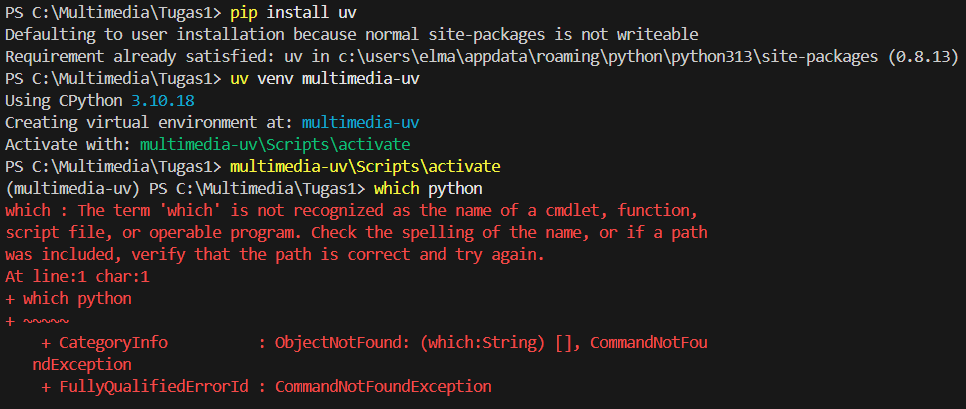
\includegraphics[scale = 0.5]{Figure/Screenshot 2025-08-28 185613.png}
    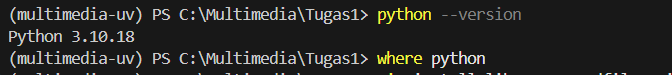
\includegraphics[scale = 0.8]{Figure/Screenshot 2025-08-28 190314.png}
	\vspace{0.1cm}
    \end{center}
\end{itemize}
    saya menggunakan "which python" terjadi eror karena perintah tersebut digunakan untuk MacOS, dan untuk windows menggunakan "where python"


\subsection{Bagian 2: Instalasi Library Multimedia}
Setelah environment aktif, install library-library berikut:

\subsubsection{Library Audio Processing}
\begin{lstlisting}[language=bash, caption=Instalasi library audio]
# Untuk conda:
conda install -c conda-forge librosa soundfile scipy

# Untuk pip (venv/uv):
pip install librosa soundfile scipy
\end{lstlisting}

\subsubsection{Library Image Processing}
\begin{lstlisting}[language=bash, caption=Instalasi library image]
# Untuk conda:
conda install -c conda-forge opencv pillow scikit-image matplotlib

# Untuk pip (venv/uv):
pip install opencv-python pillow scikit-image matplotlib
\end{lstlisting}

\subsubsection{Library Video Processing}
\begin{lstlisting}[language=bash, caption=Instalasi library video]
# Untuk conda:
conda install -c conda-forge ffmpeg
pip install moviepy

# Untuk pip (venv/uv):
pip install moviepy
\end{lstlisting}

\subsubsection{Library General Purpose}
\begin{lstlisting}[language=bash, caption=Instalasi library umum]
# Untuk conda:
conda install numpy pandas jupyter

# Untuk pip (venv/uv):
pip install numpy pandas jupyter
\end{lstlisting}

\textbf{Dokumentasikan di sini:}
\begin{itemize}
    \item Perintah instalasi yang Anda gunakan
    \item Screenshot proses instalasi atau output sukses
    \item Daftar library yang berhasil diinstall dengan versinya
    \begin{lstlisting}[language=bash, caption=Instalasi library umum]
Instalasi library audio:
    (multimedia-uv) PS C:\Multimedia\Tugas1> uv pip install librosa soundfile scipy
    Using Python 3.10.18 environment at: multimedia-uv
    Resolved 25 packages in 4.51s
    Prepared 13 packages in 8m 22s
    Installed 13 packages in 539ms
    + audioread==3.0.1                                                                                                                                              
    + joblib==1.5.2                                                                                                                                                 
    + lazy-loader==0.4                                                                                                                                              
    + librosa==0.11.0                                                                                                                                               
    + llvmlite==0.44.0                                                                                                                                              
    + msgpack==1.1.1                                                                                                                                                
    + numba==0.61.2                                                                                                                                                 
    + pooch==1.8.2                                                                                                                                                  
    + scikit-learn==1.7.1                                                                                                                                           
    + scipy==1.15.3                                                                                                                                                 
    + soundfile==0.13.1                                                                                                                                             
    + soxr==0.5.0.post1                                                                                                                                             
    + threadpoolctl==3.6.0

Instalasi library image:
    (multimedia-uv) PS C:\Multimedia\Tugas1> uv pip install opencv-python pillow scikit-image matplotlib
    Using Python 3.10.18 environment at: multimedia-uv
    Resolved 18 packages in 14.28s
    Resolved 18 packages in 14.28s
    Prepared 5 packages in 7m 22s
    Installed 12 packages in 452ms
    + contourpy==1.3.2
    + cycler==0.12.1
    + fonttools==4.59.2
    + imageio==2.37.0
    + kiwisolver==1.4.9
    + matplotlib==3.10.5
    + matplotlib==3.10.5
    + networkx==3.4.2
    + opencv-python==4.12.0.88
    + pillow==11.3.0
    + pyparsing==3.2.3
    + scikit-image==0.25.2
    + tifffile==2025.5.10

Instalasi library video:
    (multimedia-uv) PS C:\Multimedia\Tugas1> uv pip install moviepy
    Using Python 3.10.18 environment at: multimedia-uv
    Resolved 10 packages in 781ms
    Resolved 10 packages in 781ms
    Prepared 4 packages in 2m 15s
    Installed 5 packages in 926ms
    + imageio-ffmpeg==0.6.0
    + moviepy==2.2.1
    + proglog==0.1.12
    + python-dotenv==1.1.1
    + tqdm==4.67.1

Instalasi library umum:
    (multimedia-uv) PS C:\Multimedia\Tugas1> uv pip install numpy pandas jupyter
    Using Python 3.10.18 environment at: multimedia-uv
    Resolved 105 packages in 2.54s                                                                                                                                   
    Prepared 9 packages in 2m 06s
    Installed 75 packages in 2.03s
    + anyio==4.10.0                                                                                                                                                 
    + argon2-cffi==25.1.0                                                                                                                                           
    + argon2-cffi-bindings==25.1.0                                                                                                                                  
    + arrow==1.3.0                                                                                                                                                  
    + async-lru==2.0.5                                                                                                                                              
    + attrs==25.3.0                                                                                                                                                 
    + babel==2.17.0
    + beautifulsoup4==4.13.5
    + bleach==6.2.0
    + certifi==2025.8.3
    + cffi==1.17.1
    + charset-normalizer==3.4.3
    + defusedxml==0.7.1
    + fastjsonschema==2.21.2
    + fqdn==1.5.1
    + h11==0.16.0
    + httpcore==1.0.9
    + httpx==0.28.1
    + idna==3.10
    + ipywidgets==8.1.7
    + isoduration==20.11.0
    + jinja2==3.1.6
    + json5==0.12.1
    + jsonpointer==3.0.0
    + jsonschema==4.25.1
    + jsonschema-specifications==2025.4.1
    + jupyter==1.1.1
    + jupyter-console==6.6.3
    + jupyter-events==0.12.0
    + jupyter-lsp==2.3.0
    + jupyter-server==2.17.0
    + jupyter-server-terminals==0.5.3
    + jupyterlab==4.4.6
    + jupyterlab-pygments==0.3.0
    + jupyterlab-server==2.27.3
    + jupyterlab-widgets==3.0.15
    + lark==1.2.2
    + markupsafe==3.0.2
    + mistune==3.1.3
    + nbclient==0.10.2
    + nbconvert==7.16.6
    + nbformat==5.10.4
    + notebook==7.4.5
    + notebook-shim==0.2.4
    + numpy==2.2.6
    + overrides==7.7.0
    + pandas==2.3.2
    + pandocfilters==1.5.1
    + prometheus-client==0.22.1
    + pycparser==2.22
    + python-json-logger==3.3.0
    + pytz==2025.2
    + pywinpty==3.0.0
    + pyyaml==6.0.2
    + referencing==0.36.2
    + requests==2.32.5
    + rfc3339-validator==0.1.4
    + rfc3986-validator==0.1.1
    + rfc3987-syntax==1.1.0
    + rpds-py==0.27.1
    + send2trash==1.8.3
    + setuptools==80.9.0
    + pytz==2025.2
    + pywinpty==3.0.0
    + pyyaml==6.0.2
    + referencing==0.36.2
    + requests==2.32.5
    + rfc3339-validator==0.1.4
    + rfc3986-validator==0.1.1
    + rfc3987-syntax==1.1.0
    + rpds-py==0.27.1
    + send2trash==1.8.3
    + setuptools==80.9.0
    + pywinpty==3.0.0
    + pyyaml==6.0.2
    + referencing==0.36.2
    + requests==2.32.5
    + rfc3339-validator==0.1.4
    + rfc3986-validator==0.1.1
    + rfc3987-syntax==1.1.0
    + rpds-py==0.27.1
    + send2trash==1.8.3
    + setuptools==80.9.0
    + referencing==0.36.2
    + requests==2.32.5
    + rfc3339-validator==0.1.4
    + rfc3986-validator==0.1.1
    + rfc3987-syntax==1.1.0
    + rpds-py==0.27.1
    + send2trash==1.8.3
    + setuptools==80.9.0
    + rfc3339-validator==0.1.4
    + rfc3986-validator==0.1.1
    + rfc3987-syntax==1.1.0
    + rpds-py==0.27.1
    + send2trash==1.8.3
    + setuptools==80.9.0
    + sniffio==1.3.1
    + soupsieve==2.8
    + terminado==0.18.1
    + rfc3987-syntax==1.1.0
    + rpds-py==0.27.1
    + send2trash==1.8.3
    + setuptools==80.9.0
    + sniffio==1.3.1
    + soupsieve==2.8
    + terminado==0.18.1
    + send2trash==1.8.3
    + setuptools==80.9.0
    + sniffio==1.3.1
    + soupsieve==2.8
    + terminado==0.18.1
    + tinycss2==1.4.0
    + sniffio==1.3.1
    + soupsieve==2.8
    + terminado==0.18.1
    + tinycss2==1.4.0
    + tinycss2==1.4.0
    + tomli==2.2.1
    + tomli==2.2.1
    + types-python-dateutil==2.9.0.20250822
    + tzdata==2025.2
    + types-python-dateutil==2.9.0.20250822
    + tzdata==2025.2
    + uri-template==1.3.0
    + types-python-dateutil==2.9.0.20250822
    + tzdata==2025.2
    + types-python-dateutil==2.9.0.20250822
    + tzdata==2025.2
    + uri-template==1.3.0
    + urllib3==2.5.0
    + webcolors==24.11.1
    + webencodings==0.5.1
    + websocket-client==1.8.0
    + widgetsnbextension==4.0.14
    \end{lstlisting}
\end{itemize}

\subsection{Bagian 3: Verifikasi Instalasi}
Buat file Python sederhana untuk menguji semua library yang telah diinstall:
\textbf{Jalankan script dan dokumentasikan hasilnya:}

\textbf{File dan dokumentasi hasil eksekusi:}
\begin{lstlisting}[language=Python, caption=verifikasi istalasi library multimedia]
import importlib

libraries = [
    ("librosa", "Audio"),
    ("soundfile", "Audio"),
    ("scipy", "Audio"),
    ("cv2", "Image"),
    ("PIL", "Image"),
    ("skimage", "Image"),
    ("matplotlib", "Image"),
    ("moviepy", "Video"),
    ("numpy", "General"),
    ("pandas", "General"),
    ("jupyter", "General"),
]

print("Cek instalasi library multimedia:\n")

for lib, category in libraries:
    try:
        module = importlib.import_module(lib)
        version = getattr(module, "__version__", "versi tidak diketahui")
        print(f"[SUKSES] {lib} ({category}) terinstall, versi: {version}")
    except Exception as e:
        print(f"[GAGAL]  {lib} ({category}) TIDAK terinstall. ({e})")
\end{lstlisting}
\begin{center}
	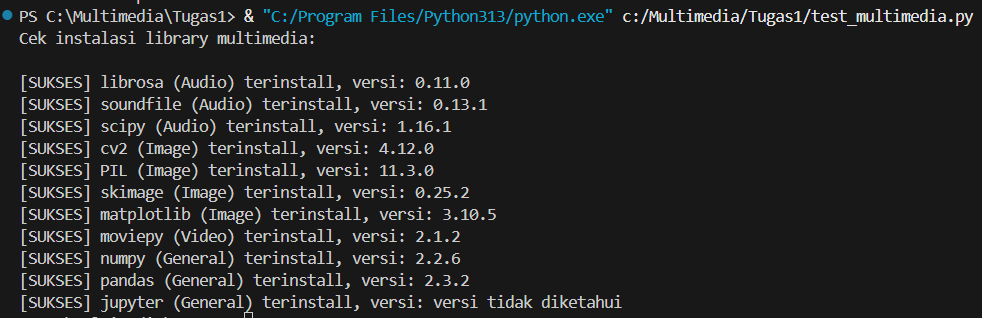
\includegraphics[scale = 0.5]{Figure/Screenshot 2025-08-28 204417.png}
	\vspace{0.1cm}
\end{center}

\subsection{Bagian 4: Simple Test dengan Sample Code}
Buat dan jalankan contoh sederhana untuk setiap kategori multimedia:

\subsubsection{Test Audio Processing}
\begin{lstlisting}[language=Python, caption=Test audio processing sederhana]
import numpy as np
import matplotlib.pyplot as plt

# Generate simple sine wave
duration = 2  # seconds
sample_rate = 44100
frequency = 440  # A4 note

t = np.linspace(0, duration, int(sample_rate * duration))
audio_signal = np.sin(2 * np.pi * frequency * t)

# Plot waveform
plt.figure(figsize=(10, 4))
plt.plot(t[:1000], audio_signal[:1000])  # Plot first 1000 samples
plt.title('Sine Wave (440 Hz)')
plt.xlabel('Time (s)')
plt.ylabel('Amplitude')
plt.grid(True)
plt.savefig('sine_wave_test.png', dpi=150, bbox_inches='tight')
plt.show()

print(f"Generated {duration}s sine wave at {frequency}Hz")
print(f"Sample rate: {sample_rate}Hz")
print(f"Total samples: {len(audio_signal)}")
\end{lstlisting}

\subsubsection{Test Image Processing}
\begin{lstlisting}[language=Python, caption=Test image processing sederhana]
import numpy as np
import matplotlib.pyplot as plt
from PIL import Image

# Create a simple test image
width, height = 400, 300
image = np.zeros((height, width, 3), dtype=np.uint8)

# Add some patterns
image[:, :width//3, 0] = 255  # Red section
image[:, width//3:2*width//3, 1] = 255  # Green section
image[:, 2*width//3:, 2] = 255  # Blue section

# Add a white circle in the center
center_x, center_y = width//2, height//2
radius = 50
Y, X = np.ogrid[:height, :width]
mask = (X - center_x)**2 + (Y - center_y)**2 <= radius**2
image[mask] = [255, 255, 255]

# Display and save
plt.figure(figsize=(8, 6))
plt.imshow(image)
plt.title('Test Image with RGB Stripes and White Circle')
plt.axis('off')
plt.savefig('test_image.png', dpi=150, bbox_inches='tight')
plt.show()

print(f"Created test image: {width}x{height} pixels")
print(f"Image shape: {image.shape}")
print(f"Image dtype: {image.dtype}")
\end{lstlisting}

\textbf{Dokumentasikan hasil eksekusi:}
\begin{itemize}
    \item Screenshot output dari kedua script di atas
    \item Gambar yang dihasilkan (sine\_wave\_test.png dan test\_image.png)
    \item Error message jika ada dan cara mengatasinya
\end{itemize}

\section{Bagian Laporan}

\subsection{Output Verifikasi Instalasi}
\textbf{Copy-paste output lengkap dari script \texttt{test\_multimedia.py} di sini:}

\begin{lstlisting}[caption=Output verifikasi instalasi]
[Cek instalasi library multimedia:

[SUKSES] librosa (Audio) terinstall, versi: 0.11.0
[SUKSES] soundfile (Audio) terinstall, versi: 0.13.1
[SUKSES] scipy (Audio) terinstall, versi: 1.16.1
[SUKSES] cv2 (Image) terinstall, versi: 4.12.0
[SUKSES] librosa (Audio) terinstall, versi: 0.11.0
[SUKSES] soundfile (Audio) terinstall, versi: 0.13.1
[SUKSES] scipy (Audio) terinstall, versi: 1.16.1
[SUKSES] cv2 (Image) terinstall, versi: 4.12.0
[SUKSES] scipy (Audio) terinstall, versi: 1.16.1
[SUKSES] cv2 (Image) terinstall, versi: 4.12.0
[SUKSES] PIL (Image) terinstall, versi: 11.3.0
[SUKSES] skimage (Image) terinstall, versi: 0.25.2
[SUKSES] skimage (Image) terinstall, versi: 0.25.2
[SUKSES] matplotlib (Image) terinstall, versi: 3.10.5
[SUKSES] moviepy (Video) terinstall, versi: 2.1.2
[SUKSES] moviepy (Video) terinstall, versi: 2.1.2
[SUKSES] numpy (General) terinstall, versi: 2.2.6
[SUKSES] pandas (General) terinstall, versi: 2.3.2
[SUKSES] jupyter (General) terinstall, versi: versi tidak diketahui]
\end{lstlisting}

\subsection{Screenshot Hasil Test}
\textbf{Sisipkan screenshot atau gambar hasil dari:}
\begin{itemize}
    \item Terminal/command prompt yang menunjukkan environment aktif
    \begin{center}
	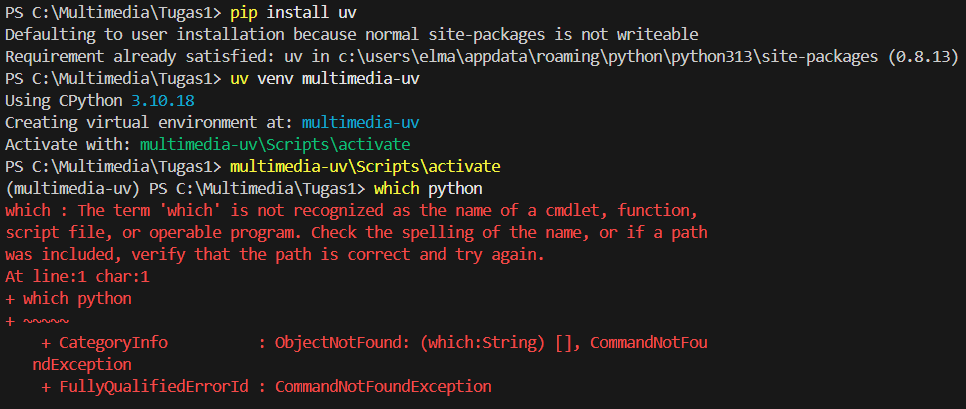
\includegraphics[scale = 0.5]{Figure/Screenshot 2025-08-28 185613.png}
    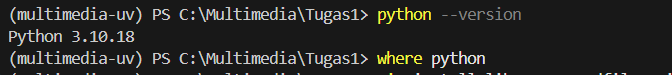
\includegraphics[scale = 0.8]{Figure/Screenshot 2025-08-28 190314.png}
	\vspace{0.1cm}
    \end{center}
    \item Output dari script test audio (sine wave plot)
    \begin{center}
	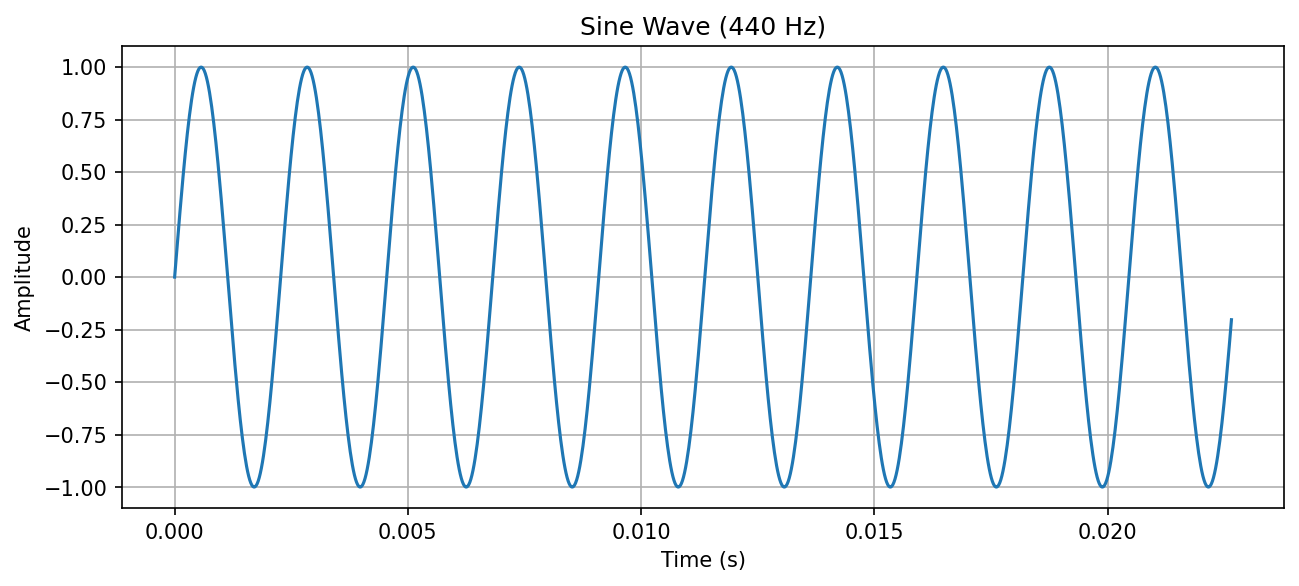
\includegraphics[scale = 0.5]{Figure/sine_wave_test.png}
    \end{center}
    \item Output dari script test image (RGB stripes dengan circle)
    \begin{center}
	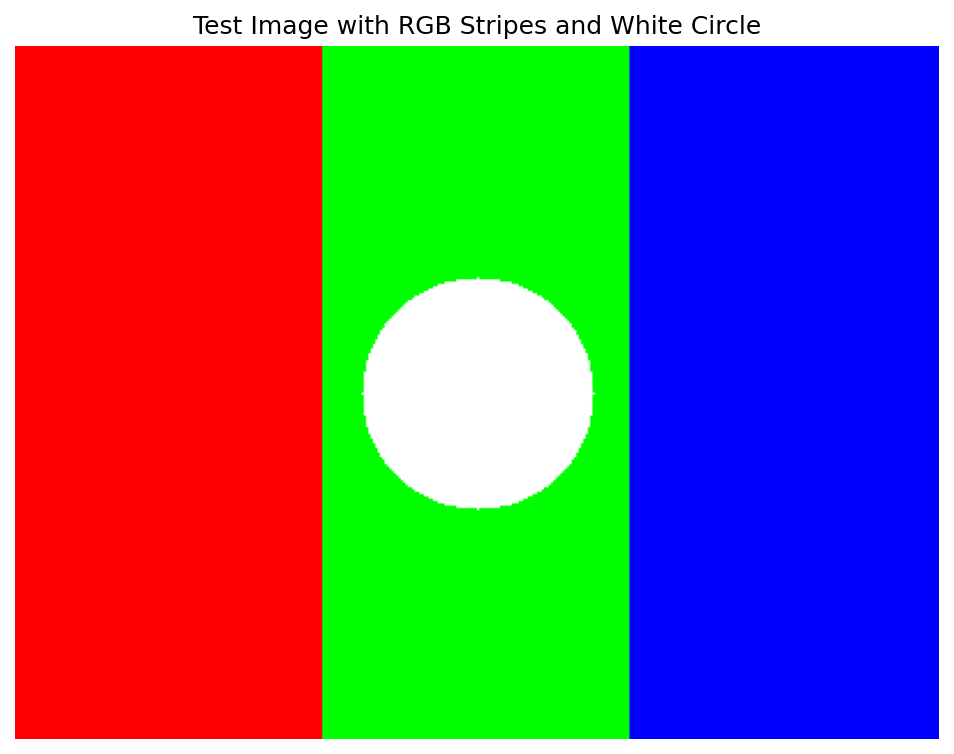
\includegraphics[scale = 0.5]{Figure/test_image.png}
    \end{center}
    \end{itemize}
    
\subsection{Analisis dan Refleksi}
\textbf{Jawab pertanyaan berikut:}

\begin{enumerate}
    \item \textbf{Mengapa penting menggunakan environment terpisah untuk project multimedia?}
    
    \textit{Menggunkana environment terpisah itu supaya tidak terjadi bentrok antar library yang dipakai. jadi semisal membuat project yang lain lagi atau yang berbeda itu tidak berpengaruh pada prpoject yang sudah pernah dibuat. kaarena tiap project itu beda beda library yang dipakai.}
    
    \item \textbf{Apa perbedaan utama antara conda, venv, dan uv? Mengapa Anda memilih tool yang Anda gunakan?}
    
    \textit{Kalau conda itu lebih lengkap dan cukup direkomendasikan untuk pemula, karena conda itu sudah include package manager dan environment manager. kalau venv itu built in python, tidak perlu install tambahan. kalau uv itu modern dan cepat tapi perlu install dulu. sayamemilih uv karena yang pertama disarankan oleh pak Martin karena lebih ringan dan cepat.}
    
    \item \textbf{Library mana yang paling sulit diinstall dan mengapa?}
    
    \textit{Kalau menurut saya sepertinya conda, karena dilihat dari proses instalasinya yang cukup panjang dan lama. mungkin karena di conda banyak package yang harus di install.}
    
    \item \textbf{Bagaimana cara mengatasi masalah dependency conflict jika terjadi?}
    
    \textit{Saya bertanya kepada chat gpt dan copilot, yang saya lakukan adalah menginstall ulang library yang bermasalah.}
    
    \item \textbf{Jelaskan fungsi dari masing-masing library yang berhasil Anda install!}
    
    \textit{Librosa untuk audio processing, soundfile untuk membaca dan menulis file audio, scipy untuk manipulasi sinyal audio, cv2 untuk image processing, PIL untuk manipulasi gambar,skimage untuk analisis gambar, matplotlib untuk visualisasi data, moviepy untuk edit video, numpy untuk komputasi numerik, pandas untuk manipulasi data, jupyter untuk notebook interaktif.}
\end{enumerate}

\subsection{Troubleshooting}
\textbf{Dokumentasikan masalah yang Anda hadapi (jika ada) dan cara mengatasinya:}

\begin{itemize}
    \item \textbf{Masalah 1:} \textit{Ketika saya menginsatll library audio, image, video, dan umum ada beberapa library yang terinstall tapi dia berada di folder yang berbeda, dia masuk di environment laptopnya bukan di environment uv.}
    
    \textbf{Solusi:} \textit{Saya bertanya kepada chat gpt terkait warning yang ada, namun kurang membantu, kemudian saya coba untuk bertanya kepada dinda, ternyata ketika menjalankan perintah "pip install ...." itu harus diawali dengan "uv" supaya dia masuk ke environment uv, jadi baru teratasi masalahnya.}
    
    \item \textbf{Masalah 2:} \textit{Ketika saya akan melakukan verifikasi environtment aktif dan mwngikuti langkah yang tertera pada dokumen ternata tidak bisa jika menggunakan "which python".}
    
    \textbf{Solusi:} \textit{Saya bertanya ke chat gpt dan mendapatkan informasi bahwa "which python" itu digunakan untuk MacOS, sedangkan untuk windows menggunakan "where python", dan akhirnya saya coba dan berhasil.}

    \item \textbf{Masalah 3:} \textit{Saya belum mahir dan familiar dengan latex, jadi dalam pembuatan dokumennya saya mengalami kesulitan.}
    
    \textbf{Solusi:} \textit{Saya hanya menggunakan code code yang sudah ada dan mengcopy paste, dan juga masih banyak yang kurang rapih menurut saya.}
\end{itemize}

\section{Export Environment untuk Reproduksi}
Sebagai langkah terakhir, export environment Anda agar dapat direproduksi:

\subsection{Untuk Conda}
\begin{lstlisting}[language=bash, caption=Export conda environment]
conda env export > environment.yml
\end{lstlisting}

\subsection{Untuk venv/uv}
\begin{lstlisting}[language=bash, caption=Export pip requirements]
pip freeze > requirements.txt
\end{lstlisting}

\textbf{Copy-paste isi file environment.yml atau requirements.txt di sini:}

\begin{lstlisting}[caption=Environment/Requirements file]
[anyio==4.10.0
argon2-cffi==25.1.0
argon2-cffi-bindings==25.1.0
arrow==1.3.0
asttokens==3.0.0
async-lru==2.0.5
attrs==25.3.0
audioread==3.0.1
babel==2.17.0
beautifulsoup4==4.13.5
bleach==6.2.0
certifi==2025.8.3
cffi==1.17.1
charset-normalizer==3.4.3
colorama==0.4.6
comm==0.2.3
contourpy==1.3.2
cycler==0.12.1
debugpy==1.8.16
decorator==5.2.1
defusedxml==0.7.1
exceptiongroup==1.3.0
executing==2.2.0
fastjsonschema==2.21.2
fonttools==4.59.2
fqdn==1.5.1
h11==0.16.0
httpcore==1.0.9
httpx==0.28.1
idna==3.10
imageio==2.37.0
imageio-ffmpeg==0.6.0
ipykernel==6.30.1
ipython==8.37.0
ipywidgets==8.1.7
isoduration==20.11.0
jedi==0.19.2
jinja2==3.1.6
joblib==1.5.2
json5==0.12.1
jsonpointer==3.0.0
jsonschema==4.25.1
jsonschema-specifications==2025.4.1
jupyter==1.1.1
jupyter-client==8.6.3
jupyter-console==6.6.3
jupyter-core==5.8.1
jupyter-events==0.12.0
jupyter-lsp==2.3.0
jupyter-server==2.17.0
jupyter-server-terminals==0.5.3
jupyterlab==4.4.6
jupyterlab-pygments==0.3.0
jupyterlab-server==2.27.3
jupyterlab-widgets==3.0.15
kiwisolver==1.4.9
lark==1.2.2
lazy-loader==0.4
librosa==0.11.0
llvmlite==0.44.0
markupsafe==3.0.2
matplotlib==3.10.5
matplotlib-inline==0.1.7
mistune==3.1.3
moviepy==2.2.1
msgpack==1.1.1
nbclient==0.10.2
nbconvert==7.16.6
nbformat==5.10.4
nest-asyncio==1.6.0
networkx==3.4.2
notebook==7.4.5
notebook-shim==0.2.4
numba==0.61.2
numpy==2.2.6
opencv-python==4.12.0.88
overrides==7.7.0
packaging==25.0
pandas==2.3.2
pandocfilters==1.5.1
parso==0.8.5
pillow==11.3.0
platformdirs==4.4.0
pooch==1.8.2
proglog==0.1.12
prometheus-client==0.22.1
prompt-toolkit==3.0.52
psutil==7.0.0
pure-eval==0.2.3
pycparser==2.22
pygments==2.19.2
pyparsing==3.2.3
python-dateutil==2.9.0.post0
python-dotenv==1.1.1
python-json-logger==3.3.0
pytz==2025.2
pywin32==311
pywinpty==3.0.0
pyyaml==6.0.2
pyzmq==27.0.2
referencing==0.36.2
requests==2.32.5
rfc3339-validator==0.1.4
rfc3986-validator==0.1.1
rfc3987-syntax==1.1.0
rpds-py==0.27.1
scikit-image==0.25.2
scikit-learn==1.7.1
scipy==1.15.3
send2trash==1.8.3
setuptools==80.9.0
six==1.17.0
sniffio==1.3.1
soundfile==0.13.1
soupsieve==2.8
soxr==0.5.0.post1
stack-data==0.6.3
terminado==0.18.1
threadpoolctl==3.6.0
tifffile==2025.5.10
tinycss2==1.4.0
tomli==2.2.1
tornado==6.5.2
tqdm==4.67.1
traitlets==5.14.3
types-python-dateutil==2.9.0.20250822
typing-extensions==4.15.0
tzdata==2025.2
uri-template==1.3.0
urllib3==2.5.0
wcwidth==0.2.13
webcolors==24.11.1
webencodings==0.5.1
websocket-client==1.8.0
widgetsnbextension==4.0.14
]
\end{lstlisting}

\section{Kesimpulan}
\textbf{Tuliskan kesimpulan Anda mengenai:}
\begin{itemize}
    \item Pengalaman setup Python environment untuk multimedia
    \item Persiapan untuk project multimedia selanjutnya
    \item Saran untuk mahasiswa lain yang akan melakukan setup serupa
\end{itemize}

\textit{Kesimpulan yang saya dapatkan adalah ketika melakukan setup python environment untuk multimedia bisa dibilang tidak mudah dan tidak sulit, mudahnya karena sudah diberikan tutorial oleh pak Martin dan sulitnya ketika mengalami touble shooting yang tidak bisa di atasi oleh AI dan diri sendiri. Untuk persiapan selanjutnya saya akan lebih teliti dan tidak panik jika mengalami eror. Dan saran untuk teman-teman yang lain jika ingin melakukan setup serupa kalau bisa mengerjakannya bersama teman, jadi bisa saling membantu dan sama-sama belajar.}

\section{Referensi}
Sertakan referensi yang Anda gunakan selama proses setup dan troubleshooting.

\newpage
\bibliographystyle{IEEEtran}
\bibliography{Referensi}
Chat GPT : https://chatgpt.com/share/68b0606a-78f8-8005-9ad0-2e6ed9927302
\end{document}